\documentclass{article}

\usepackage{lmodern}
\usepackage{hyperref}
\usepackage{amsmath}
\usepackage{amssymb}
\usepackage[T1]{fontenc}
\usepackage{fancyhdr}
\usepackage{color,graphicx}
\pagestyle{fancy}
\lhead{Anirudhan J. Rajagopalan --- ajr619}
\lhead{Michele Ceru --- mc3784}

\begin{document}

\title{Deep Learning --- Homework 2}
\date{February 11, 2016}
\author{Anirudhan J. Rajagopalan, Michele Ceru\\ ajr619, mc3784}

\maketitle

\newpage

\section[Expression for energy]{More Backpropogation}
\subsection{Backpropagation through a DAG of modules}
Defining the vectors $o=(o_{max},o_{min})$, $x=(x_1,x_2)$ and $\frac{\partial E}{\partial x} =(\frac{\partial E}{\partial x_1},\frac{\partial E}{\partial x_2}  )$ the first step in back propagation is:

$$
\frac{\partial E}{\partial o} =\frac{\partial E}{\partial y} \frac{\partial y}{\partial o}=(\frac{\partial E}{\partial y} ,\frac{\partial E}{\partial y} )
$$
The second step:
$$
\frac{\partial E}{\partial i} = \frac{\partial E}{\partial o} \frac{\partial o}{\partial i} =
(\frac{\partial E}{\partial y} ,\frac{\partial E}{\partial y} )
\begin{bmatrix}
 \frac{\partial max(i_1,i_2)}{\partial i_1}     & \frac{\partial max(i_1,i_2)}{\partial i_2}\\
\frac{\partial min(i_1,i_2)}{\partial i_1}     & \frac{\partial min(i_1,i_2)}{\partial i_2}   \\
\end{bmatrix}=
(\frac{\partial E}{\partial y} ,\frac{\partial E}{\partial y} )
\begin{bmatrix}
1 & 0\\
0 & 1  \\
\end{bmatrix}=(\frac{\partial E}{\partial y} ,\frac{\partial E}{\partial y} )
$$
Finally:
$$
\frac{\partial E}{\partial x}= \frac{\partial E}{\partial i} \frac{\partial i}{\partial x}=
(\frac{\partial E}{\partial y} ,\frac{\partial E}{\partial y} )
\begin{bmatrix}
\frac{\partial \sigma_1}{\partial x_1} & \frac{\partial \sigma_1}{\partial x_2}\\
\frac{\partial \sigma_2}{\partial x_1} & \frac{\partial \sigma_2}{\partial x_2} \\
\end{bmatrix}=
(\frac{\partial E}{\partial y} ,\frac{\partial E}{\partial y} )
\begin{bmatrix}
\frac{e^{-x_1}}{(1+e^{-x_1})^2}&0\\
0&\frac{e^{-x_2}}{(1+e^{-x_2})^2} \\
\end{bmatrix}
$$ 
That is:
\begin{eqnarray*}
\frac{\partial E}{\partial x_1}&=&\frac{\partial E}{\partial y}\frac{e^{-x_1}}{(1+e^{-x_1})^2},\\
\frac{\partial E}{\partial x_2}&=&\frac{\partial E}{\partial y}\frac{e^{-x_2}}{(1+e^{-x_2})^2}
\end{eqnarray*}

\subsection{Batch Normalization}
\paragraph{1:} Using the chain rule we have:
$$
\frac{\partial E}{\partial x_k}=\frac{\partial E}{\partial y_k}\frac{\partial y_k}{\partial x_k}+
\frac{\partial E}{\partial E(x_k)}\frac{\partial E(x_k)}{\partial x_k}+
\frac{\partial E}{\partial \sigma^2(x_k)}\frac{\partial \sigma^2(x_k)}{\partial x_k}=
$$
and so:
\begin{equation}\label{backprop}
\frac{\partial E}{\partial x_k}=\frac{\partial E}{\partial y_k}\frac{1}{\sqrt{	\sigma^2(x_k)}}+\frac{\partial E}{\partial E(x_k)}	\frac{1}{n}+
\frac{\partial E}{\partial \sigma^2(x_k)}\frac{2}{n}	\sum_{i=1}^{n}(x_{k_i}-E(x_k))
\end{equation}
where we used the definition of $E(x_k)$ and $\sigma(x_k)$ to calculate their derivatives. And where:
$$
\frac{\partial E}{\partial E(x_k)}=\sum_{i=1}^n \frac{\partial E}{	\partial y_{k_i}}
\frac{\partial y_{k_i}}{{\partial E(x_k)}}+
\frac{\partial E}{	\partial\sigma^2(x_k)}
\frac{\sigma^2(x_k)}{{\partial E(x_k)}}=
\sum_{i=1}^n \frac{\partial E}{	\partial y_{k_i}}	\frac{-1}{\sqrt{	\sigma^2(x_k)}}+
\frac{\partial E}{	\partial\sigma^2(x_k)}(\frac{-2}{n}\sum_{i=1}^n(x_{k_i} -E(x_k)))
$$
$$
\frac{\partial E}{	\partial\sigma^2(x_k)}=
\sum_{i=1}^n \frac{\partial E}{\partial y_{k_i}}
\frac{\partial y_{k_i}}{{\partial \sigma^2(x_k) }}=
\sum_{i=1}^n \frac{\partial E}{\partial y_{k_i}}	\big[-\frac{1}{2\sqrt{(\sigma^2(x_k))^3}} (x_{k_i}-E(x_k))\big]
$$
\paragraph{2:}Adding a learnable bias we have:
$$
y_k=	\frac{x_k-E(x_k)}{\sqrt{\sigma^2(x_k)}}+\epsilon
$$ 
The back propagation will be the same of (\ref{backprop}). And in addition we have the parameter $\epsilon$ for which:
$$
\frac{\partial E}{\partial \epsilon}=\sum_{i=0}^{n}\frac{\partial E}{\partial y_{k_i}}\frac{ \partial y_{k_i}}{\partial \epsilon}=
\sum_{i=0}^{n}\frac{\partial E}{\partial y_{k_i}}
$$

\section{Visualization}
\begin{centering}
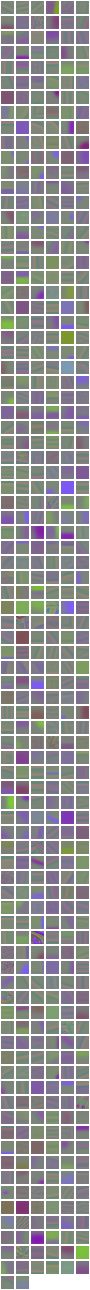
\includegraphics[scale=0.5]{images/centroids.png}
\end{centering}


\begin{centering}
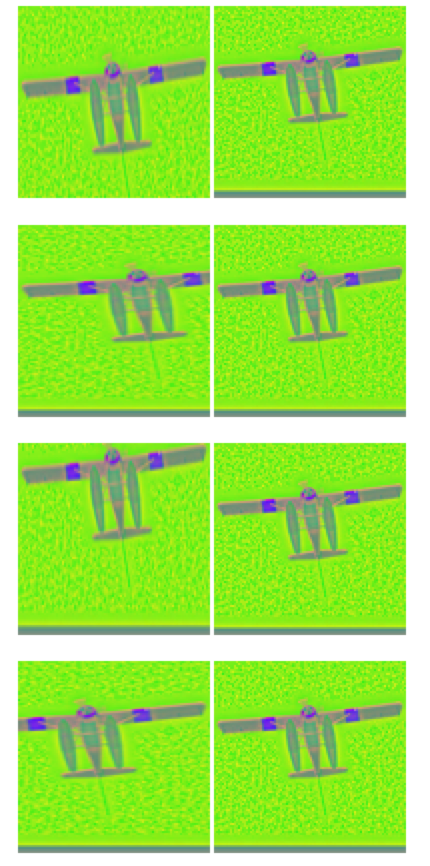
\includegraphics[scale=0.5]{images/ImageDistortion.png}
\end{centering}

\section{Kaggle}

%Kmeans folder
\begin{centering}
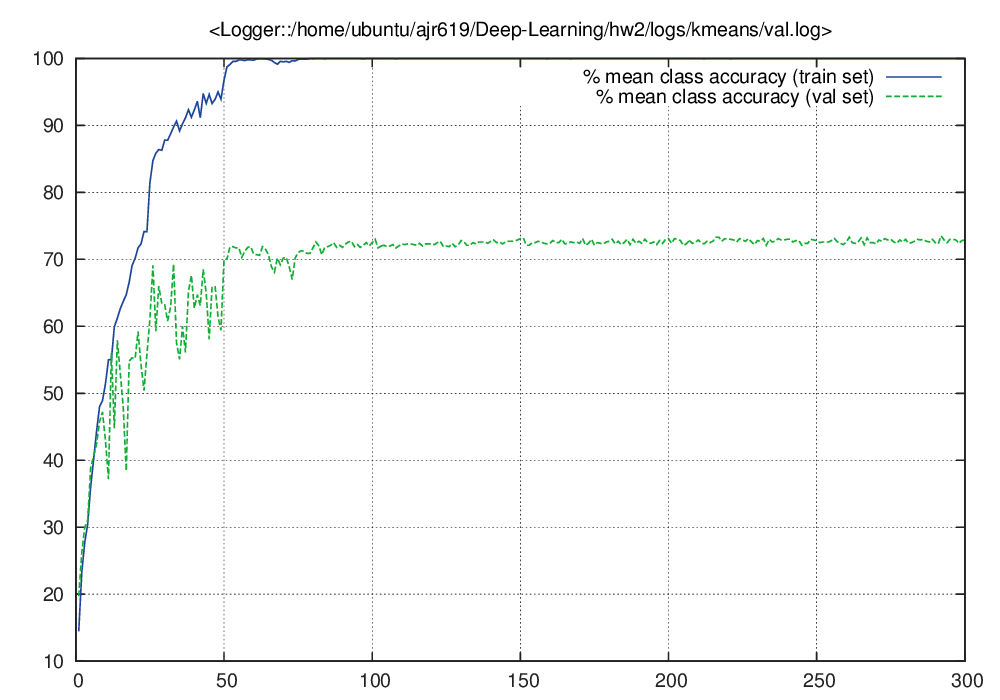
\includegraphics[scale=0.3]{images/kmeans/val.png}
\end{centering}

%Kmeans.1 folder
\begin{centering}
\includegraphics[scale=0.3]{images/kmeans.1/val.png}
\end{centering}

%vgg folder
\begin{centering}
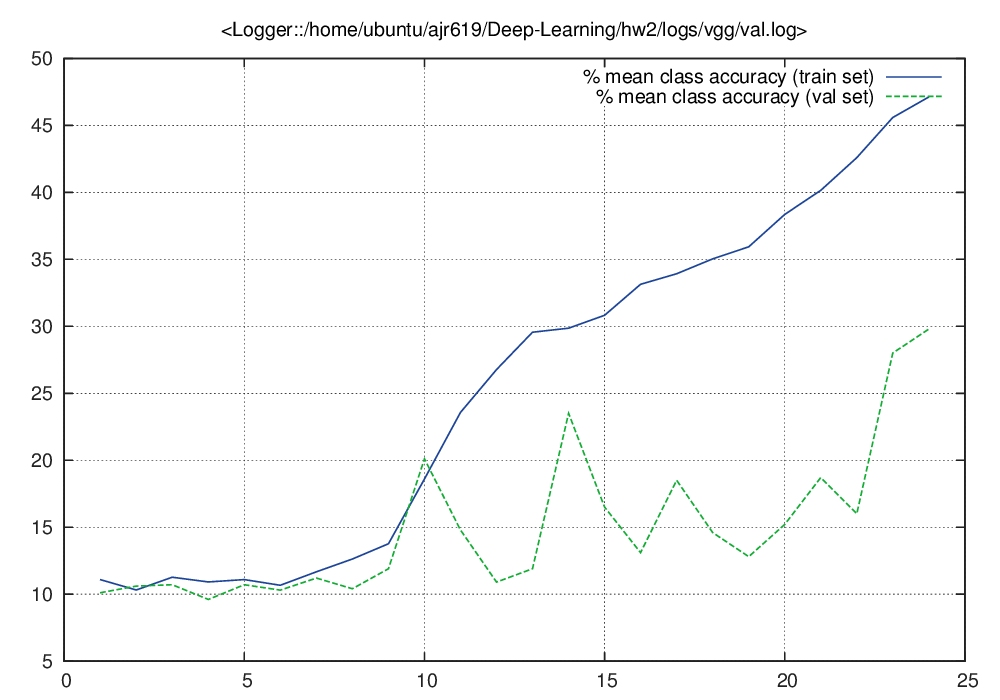
\includegraphics[scale=0.3]{images/vgg/val.png}
\end{centering}

%vgg folder in path:/home/ubuntu/ajr619/ds-ga-1008-a2/logs
\begin{centering}
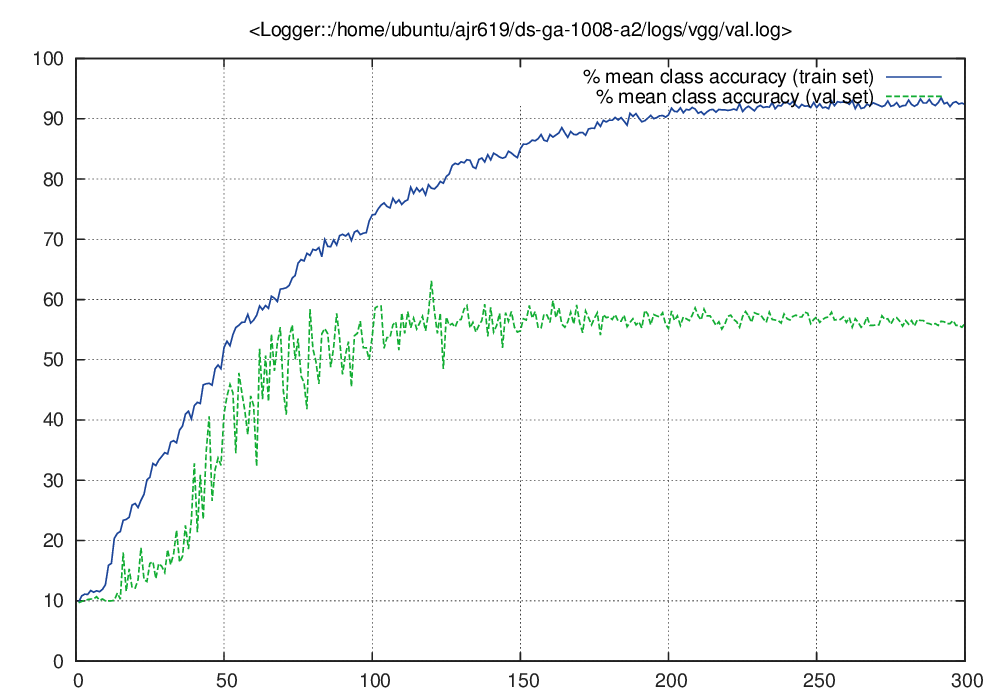
\includegraphics[scale=0.3]{images/vggInDS-ga/val.png}
\end{centering}

%/home/ubuntu/ajr619/ds-ga-1008-a2/logs_default
\begin{centering}
\includegraphics[scale=0.3]{images/logs_default/val.png}
\end{centering}



\end{document}

